\scanpage{48}
% archive sheet number: 47

\unsure{7|2}.2.1984

\uline{Structure de $K$} On rajoute des sommets d'ordre 2, soit $S_K$ l'ens des sommets. On désigne par $K$ le graphe top. avec ses nouveaux sommets. (les anciens sont ceux de l'\deleted{$K$}ordre 4). On a

\[ S_K=\underbrace{S'_K}_{\substack{\text{sommets}\\\text{rouges}}}\amalg
\underbrace{S''_K}_{\substack{\text{sommets}\\\text{\deleted{rouges}\inserted{noirs}}}} \]

\margin{\uline{NB} \deleted{$I$ \unsure{et} $S_K$ \unsure{que} $S''$} \inserted{$S'_K$ contient des} sommets d'ordre 2, pas néc. des sommets d'ordre 4 $S''_K$ contient des sommets d'ordre 2 pas néc. d'ordre 4}

avec :

a) Pour tte \deleted{\illegible{1}} face $F$, $S'_K\cap F$ et $S''_K\cap F\unsure{_2}$ st des subdivisions de $\partial F$ duales l'une de l'autre, d'ordre $2n$

\deleted{\unsure{b)}} \uline{NB} --- Deux sommets consécutifs sur $\partial F$ ne sont pas d'ordre 4, et \deleted{plus} précisément, \deleted{\unsure{entre deux}} sur un arc de $\partial F$ joignant deux sommets d'ordre 4, il y a toujours au moins un sommet rouge d'ordre 2, (et même deux si $\Sigma$ n'est pas \deleted{d'ordre} du type $\mathrm{II}_p$ et on est sur une arête exceptionnelle) et au moins un sommet noir (si on n'est \unsure{B}| par tous les cas qu'on vient de dire\ldots)

b) \deleted{Intro} On a une section du fais des visées pour le déploiement $K'$ de $K$. Ainsi, chaque arête $a$ d'une face \inserted{$F$} est munie d'un signe $\varepsilon_F(a)$, qui est \deleted{\unsure{$\pm$}}$+1$ si la visée est du côté de $F$, $-1$ sinon. On a les règles

\[
\left\{\begin{aligned}
\varepsilon_{F'}(\unsure{a'})&=-\varepsilon_F(a) &&\text{si $F,F'$ sont les deux faces incidentes à $a$}\\
\varepsilon_F(\unsure{a})&=\varepsilon_{\unsure{F}}(\unsure{b}) &&\text{si $a$ et $b$ sont adjacentes sur $F$, le sommet commun étant d'ordre 2}\\
\varepsilon_{a_1}(F_1)&=\varepsilon_{a_2}(F_2) &&\text{si $F_1$ et $F_2$ sont adjacentes le long d'une}\\[-2pt]
&&&\text{arête mitoyenne $b$, d'extrémité $s$, d'ordre 4}\\
&&&\text{et quand $a_1$ et $a_2$ sont incidentes à $F_1$ et $F_2$}\\
&&&\text{respectivement, $\ne b$, et incidentes à $s$.}
\end{aligned}\right.
\]

\figure{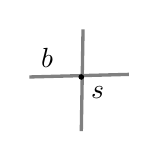
\begin{tikzpicture}[scale=.55]\draw[gray,very thick] (-1.2,0)--(1.1,.06) (0,-1.25)--(.04,1.1);\fill (0,0) circle (.065);\node[above] at (-.79,0){$b$};\node[below right] at (0,0){$s$};\end{tikzpicture}}

Il résulte du fait que \deleted{\unsure{l tes}} les faces sont de même ordre $4n$, que pour \deleted{deux arêt} toute arête $a$, si $F,F'$ sont les deux faces incidentes, on a une \unsure{som|sorte} de \uline{symétrie autour de $a$}

\margin{\uline{NB} on a $\sigma_a^F\sigma_a^{F'}=\mathrm{id}$}

\[ \sigma_a^F\text{ ou }\sigma_a:\quad \deleted{\unsure{F}}\operatorname{Pol}(F)\xrightarrow{\sim}\operatorname{Pol}(F') \]

caractérisé par la condition de laisser \deleted{invariants} \inserted{fixes} les deux extrémités de $a$. Il laisse alors \deleted{invariants} \inserted{fixes} \deleted{toutes} tous les sommets et arêtes qui sont sur la ``grande arête'' $\widehat a$ contenant $a$ (bordée par les sommets d'ordre 4 les plus proches) (mais \deleted{pas les \unsure{prochai}} \inserted{les prochains sommets sur $\partial F$} (de part et d'autre de $\widehat a$ sont non fixés par $\sigma_a$). L'application $\sigma_a$ transforme sommets rouges (resp. noirs) en sommets noirs

% slanted
\margin{\uline{NB} $\sigma_a^F=\sigma_{a'}^F$ si $a$, $a'$ sont sur la même \uline{grande arête}}
